
% Injection {{{ %
\begin{frame}[<+->]
  \frametitle{Injection/Surjection/Bijection}
  \begin{block}{Définition}
  Soit $E$ et $F$ deux ensembles et $f:E\rightarrow F$ une application.
  L'application $f$ est dite \textbf{\alert{injective}} si:

  \begin{equation}
    \forall x_1,x_2 \in E\quad \big(  f(x_1) = f(x_2) \implies x_1= x_2\big)
  \end{equation}


\end{block}  

      \begin{center}   
        \begin{tikzpicture}
   \node[ellipse, minimum width=1.5cm, minimum height=2.5cm, draw,
     thick, label=left:$E$] at(0,0)  {};
   \node[ellipse, minimum width=1.5cm, minimum height=2.5cm, draw,
     thick, label=right:$F$] at(3,0)  {};
   \node[point] (A) at (0.2,0.5){};
   \node[point] (B) at (0.1,0.0){};
   \node[point] (C) at (-0.15,-0.4){};

   \node[point, fill=Apricot,xshift=3cm ] (fA) at (0.2,0.5){};
   \node[point, fill=Apricot,xshift=3cm] (fB) at (0.1,0.0){};
   \node[point, fill=Apricot,xshift=3cm] (fC) at (0.15,-0.6){};
   \node[point, fill=Apricot,xshift=3cm] (fD) at (0,-0.8){};

   \path[->,>=stealth, thick] (A) edge[bend left=45] (fA);
   \path[->,>=stealth, thick] (B) edge[bend left=35] (fB);
   \path[->,>=stealth, thick] (C) edge[bend left=25] (fC);
 \end{tikzpicture}
 \end{center}

  \begin{itemize}
    \small
  \item Formuler l'injectivité en utilisant la notion
    d'\textbf{\alert{antécedent}}?
  \end{itemize}
\end{frame}
% }}} Injection %
% Surjection {{{ %

\begin{frame}[<+->]
  \frametitle{Surjection}
  \begin{block}{Définition}
  Soit $E$ et $F$ deux ensembles et $f:E\rightarrow F$ une application.
  L'application $f$ est dite \textbf{\alert{surjective}} si:

  \begin{equation}
    \forall y \in F\quad \exists x\in E   \left(y = f(x)\right)
  \end{equation}


\end{block}  


\begin{columns}
  \begin{column}{0.5\textwidth}
    
      \begin{center}   
        \begin{tikzpicture}
   \node[ellipse, minimum width=1.5cm, minimum height=2.5cm, draw,
     thick, label=left:$E$] at(0,0)  {};
   \node[ellipse, minimum width=1.5cm, minimum height=2.5cm, draw,
     thick, label=right:$F$] at(3,0)  {};
   \node[point] (A) at (0.2,0.5){};
   \node[point] (B) at (0.1,0.0){};
   \node[point] (C) at (-0.15,-0.4){};
   \node[point ] (D) at (0,-0.8){};

   \node[point, fill=Apricot,xshift=3cm ] (fA) at (0.2,0.5){};
   \node[point, fill=Apricot,xshift=3cm] (fB) at (0.1,0.0){};
   \node[point, fill=Apricot,xshift=3cm] (fC) at (0.15,-0.6){};

   \path[->,>=stealth, thick] (A) edge[bend left=45] (fA);
   \path[->,>=stealth, thick] (B) edge[bend left=35] (fB);
   \path[->,>=stealth, thick] (C) edge[bend left=25] (fC);
   \path[->,>=stealth, thick] (D) edge[bend left=25] (fC);
 \end{tikzpicture}
 \end{center}
  \end{column}
  \begin{column}{0.5\textwidth}
   \begin{center}
     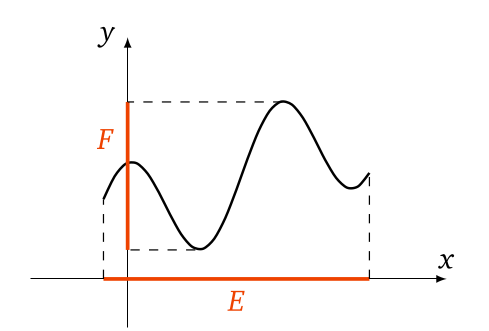
\includegraphics[width=4.5cm, height=3.5cm]{./surjection.png}
   \end{center} 
  \end{column}
\end{columns}

  \begin{itemize}
    \small
  \item Formuler la surjectivitié en utilisant la notion
    d'\textbf{\alert{antécedent}}?
  \end{itemize}

\end{frame}


\begin{frame}[<+->]
  \frametitle{Tester vos connaissances}

  \begin{columns}
    \begin{column}{0.5\textwidth}
      \only<1->{

        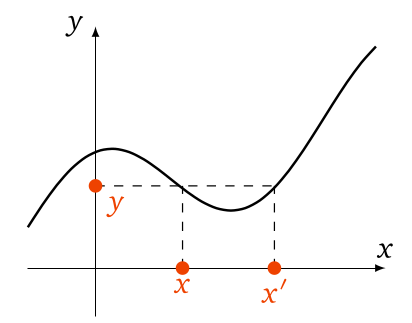
\includegraphics[width=4cm, height=4cm]{./injectivit_q1.png}
      } 

      \only<2->
      {

        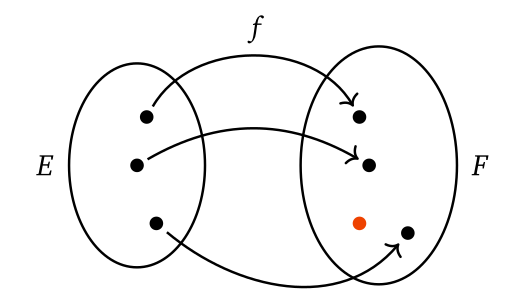
\includegraphics[width=4cm, height=4cm]{./injectivit_q2.png}
      }
    \end{column}
    \begin{column}{0.5\textwidth}
      
      \only<3->
      {

        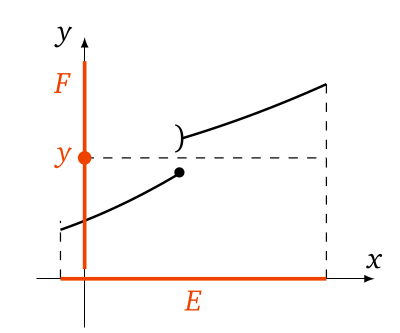
\includegraphics[width=4cm, height=4cm]{./injectivit_q3.png}
      }

      \only<4->
      {

        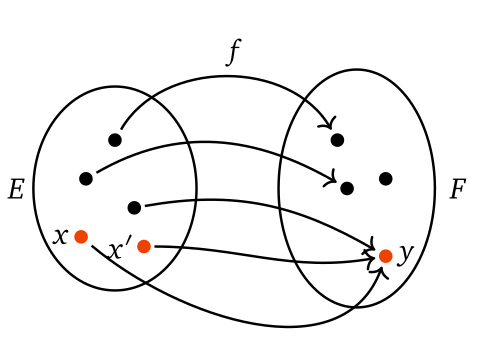
\includegraphics[width=4cm, height=4cm]{./injectivit_q4.png}
      }
    \end{column}
  \end{columns}
  
\end{frame}


\begin{frame}[t]
  \frametitle{Exercices rapides}
 \begin{block}{Exemple 1}
   Domontrer que la fonction $f: \N\rightarrow \Q$ définie par $f(n) =
   \dfrac{1}{n+1}$ est \textbf{injective}. 
 \end{block} 
 \begin{block}{Exemple 2}
   Démonter par \textbf{\alert{contre exemple}}  que la fonction $x^3$ n'est pas
   \textbf{injective}.
 \end{block}

 \begin{block}{Exemple 3}
   
   La fonction $g:\R\rightarrow\R$ est elle \textbf{\alert{surjective}}?
 \end{block}
\end{frame}
% }}} Surjection %
% Bijection {{{ %
\begin{frame}[t]
  \frametitle{Injectivité}
 \begin{block}{Définition}
   Une fonction $f:E\rightarrow F$ est dite \textbf{\alert{bijective}} si elle est injective et
   surjective. Cela revient à dire que:

   \begin{equation}
     \forall y\in F\quad \alert{\exists!} x \in E \quad \left( y = f(x)\right)
   \end{equation}
 \end{block} 

 \begin{columns}
   \begin{column}{0.5\textwidth}

      \begin{center}   
        \begin{tikzpicture}
   \node[ellipse, minimum width=1.5cm, minimum height=2.5cm, draw,
     thick, label=left:$E$] at(0,0)  {};
   \node[ellipse, minimum width=1.5cm, minimum height=2.5cm, draw,
     thick, label=right:$F$] at(3,0)  {};
   \node[point] (A) at (0.2,0.5){};
   \node[point] (B) at (0.1,0.0){};
   \node[point] (C) at (-0.15,-0.4){};

   \node[point, fill=Apricot,xshift=3cm ] (fA) at (0.2,0.5){};
   \node[point, fill=Apricot,xshift=3cm] (fB) at (0.1,0.0){};
   \node[point, fill=Apricot,xshift=3cm] (fC) at (0.15,-0.6){};

   \path[->,>=stealth, thick] (A) edge[bend left=45] (fA);
   \path[->,>=stealth, thick] (B) edge[bend left=35] (fB);
   \path[->,>=stealth, thick] (C) edge[bend left=25] (fC);
 \end{tikzpicture}
 \end{center}
     
   \end{column}
   \begin{column}{0.5\textwidth}
     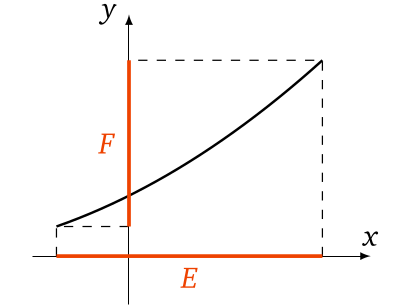
\includegraphics[width=4cm, height=4cm]{./bijective.png}  
   \end{column}
 \end{columns}
\end{frame}

\begin{frame}[t]
  \frametitle{Résultat Bijection}
  \normalsize
  \begin{block}{Proposition}
    Soit $E$, $F$ deux ensembles et $f: E\rightarrow F$ une application.

    \begin{enumerate}
      \item L'application $f$ est bijective si et seulement si il existe une
        application $g:F\rightarrow E$ telle que:
        \begin{itemize}
          \item $f\circ g=\text{id}_F$ 
          \item  $g\circ f = \text{id}_E$.
        \end{itemize}
      \item Si $f$ est bijective alors l'application $g$ est
        \textbf{\alert{unique}}  et elle est aussi bijective.
    \end{enumerate}
 \end{block}  

 \begin{itemize}
   \item L'applicaiton $g$ s'appelle \textbf{\alert{bijection réciproque}} de
     $f$ est elle est notée $f^{-1}$. On vérifie que $(f^{-1})^{-1}= f$
 \end{itemize}
 \begin{block}{Exemple}
   La bijection réciproque de la fonction 
   $f:R\rightarrow ]0,\infty[$ par $f(x)= \exp(x)$
  est la fonction $g: ]0,\infty[ \rightarrow \R$ par $g(x)=ln(x)$
 \end{block}
\end{frame}

\begin{frame}[t]
  \frametitle{Résultat Bijection}

  \begin{block}{Proposotion}
 Soit $f: E\rightarrow F$ et $ g:F\rightarrow G$ deux applications.
 \begin{itemize}
   \item Si les deux applications $f$ et $g$ sont injectives, alors $g\circ f$
     est injective.   

   \item Si les deux applications $f$ et $g$ sont surjectives, alors $g\circ f$
     est surjective.   
   \item  Ainsi si, $f$ et $g$ sont bijectives, alors $g\circ f$ est bijective.
 \end{itemize}

  \end{block}


 Alors l'application $(g\circ f)$ est \textbf{\alert{bijective}}. Sa bijection
 réciproque est donnée par:
 \begin{equation}
   \left(g\circ f\right)^{-1} = f^{-1}\circ g^{-1}
 \end{equation}
\end{frame}

  \begin{frame}[t]
    \frametitle{Mini Exercices}
    \begin{itemize}
      \item Les fonctions suivantes sont-elles injectives, surjectives,
        bijectives?

        \begin{enumerate}
          \item $f_1: \R\rightarrow [0,\infty[$, $f_1(x)=x^2$.\\[6pt]
          \item $f_2: [0,\infty]\rightarrow [0,\infty[$, $f_2(x)=x^2$.\\[6pt]
          \item $f_3: \N\rightarrow \N$, $f_3(n)=n^2$.\\[6pt]
          \item $f_4: \Z\rightarrow \Z$, $f_4(n)=n-7$.\\[6pt]
          \item $f_5: \R\rightarrow [0,\infty]$, $f_5(x)=\vert x\vert$.\\[6pt]
        \end{enumerate}
      \item Montrer que la fonction $f:]1,\infty[ \rightarrow ]0,\infty[$
        définie par $f(x)= \dfrac{1}{x-1}$ est bijective. Calculer sa bijection
        réciproque.
    \end{itemize} 
  \end{frame}
% }}} Bijection %
